\section{Unsupervised Domain Adaptation via I2I Translation}
\subsection{Introduction}
\paragraph{}
In the application of computer vision model, the ability of domain shift is seen as an important evaluation index. Because supervised models are usually trained under pairs of training image set and corresponding labels. However, there exists plenty of wild images with different distribution and patterns from training set. That's say these models may only perform well in limited domain. And if we want to obtain a model with enough versatility, we need to include enough images and label them for the training. That's a big cost. So researchers are trying to find a way to implement one model with limited data and adapt it to other domains.

The idea of Cycada\cite{cycada} is to apply unsupervised domain adaption(UDA) to images semantic segmentation to improve its versatility. They first use image-to-image translation mode to implement domain shift on training set. Then they train two image semantic segmentation model. One is on original training domain and label, another is on target domain with original label. The second model have better performance on semantic segmentation task in target domain. By mapping source domain to target domain, we find a way to adapt model to other tasks without additional labeling.

In the first task we implement the unpaired stylish image translation between GTA5 set and Cityscape set. In the second task we utilize the translation results to train the semantic segmentation model, and compare its performance on target domain with the model trained on source image and label. 

\subsection{DeepLabV3}
\paragraph{}
The model we use for semantic segmentation is DeepLabV3\cite{2017Rethinking}. The author of DeepLabV3 wants to solve two chanllenges in application of DCNN to the field of semantic segmentation. The first one is the reduced feature resolution caused by consecutive pooling operations or convolution striding. This invariance to local image transformation may impede dense prediction tasks, where detailed spatial information is desired. Another is the poor performance in detecting multiple objects at different scales. To solve them, the paper proposes Atrous Spatial Pyramid Pooling(ASPP) in DeepLabV3.

\subsubsection{Atrous Convolution}
\paragraph{}
Atrous convolution is a technique widely applied in semantic segmentation, also known as dilated convolution. It can help extract denser feature maps by removing the downsampling operations from the last few layers and upsampling the corresponding filter kernels, equivalent to inserting holes between filter weights. Atrous convoltion allows us to effectively enlarge the field of view of filters to incorporate multi-scale context\cite{dilatedcon} without expanding computation.

\begin{figure}
    \centering
    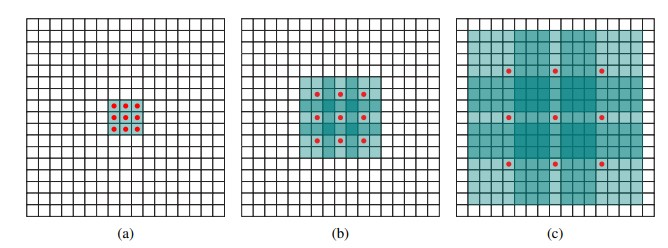
\includegraphics{Section3/dilated convolution.jpg}
    \caption{Systematic atrous supports exponential expansion of the receptive field without loss of resolution or coverage}
    \label{fig:dilated}
\end{figure}

\subsubsection{Atrous Spatial Pyramid Pooling}
\paragraph{}
Atrous Spatial Pyramid Pooling is Spatial Pyramid Pooling(SPP) combined with atrous convolution. SPP was first proposed to handle the issue that convolution network can only get fix-sized images\cite{spp}. It proved to be an effective way to resample features at different scales for accurately and efficiently classifying regions of an arbitrary scale. In DeepLabV3, author explore atrous convolution as a context module and tool for spatial pyramid pooling, and add batch normalize to the model. To solve the filter degeneration problem and incorporate global context information to the model, image-level features are adopted, as shown in Fig \ref{fig:aspp}.

\begin{figure}
    \centering
    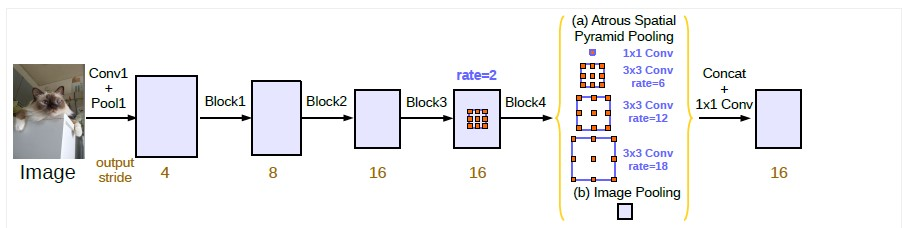
\includegraphics[width=0.8\textwidth]{Section3/aspp.jpg}
    \caption{Parallel modules with ASPP, augmented with image-level features.}
    \label{fig:aspp}
\end{figure}

\subsection{Implementation}
\paragraph{}
Our implementation of DeepLab V3 is largely based on~\cite{Deeplab}, and we make some adaptations in order to train the model on our dataset. As code for testing is not included in~\cite{Deeplab}, we also implement a script for model testing. The pseudo code for the overall procedure of training, validation and testing is shown in Algorithm~\ref{alg:deeplab}, and the details will be discussed in following sections.
\begin{algorithm}[!ht]
    \caption{Overall procedure for Semantic Segmentation}\label{alg:deeplab}
    \textbf{Objective}: Train a semantic segmentation model and evaluate performance\\
    \textbf{Input}: Training set $train\_set$, validation set $val\_set$, testing set $test\_set$\\
    \textbf{Parameter}: Parameter sets, including training epoch $e$.
    \begin{algorithmic}[1]
        \STATE~Load $train\_set$, $val\_set$, $test\_set$ and perform pre-processing.
        \STATE~Initialize the DeepLab model $M$.
        \FOR{$i=1,2,...,e$}
            \STATE~Train $M$ on $train\_set$.
            \STATE~Validate $M$ on $val\_set$, evaluate with evaluation metrics.
            \IF{$M$ is the best model in validation so far}
                \STATE~Save parameters of $M$. 
            \ENDIF{}
        \ENDFOR{}
        \STATE~Load the best model $M$.
        \STATE~Evaluate $M$ on $test\_set$ with evaluation metrics.
        \STATE~Save processed images.
    \end{algorithmic}
\end{algorithm}
\subsubsection{Dataset \& Pre-processing}
\paragraph{}
The source-only model use original GTA5 dataset from~\cite{richter2016playing} for training and validation, and use cityscape dataset from~\cite{cordts2016cityscapes} for testing. On the other hand, the domain adaptive semantic segmentation model is trained on translated cityscape-style GTA5 images obtained from the first task, and also evaluated on cityscape dataset.

As GTA5 and cityscape dataset share the same label domain, we follow the pre-processing procedure for cityscape in~\cite{Deeplab}. We define three dataloaders to load datasets: train\_loader, val\_loader and test\_loader. For training images and labels, we perform random flip, crop and gaussian blur, and normalize with given parameters. For validation and testing sets, we adjust the size of images and labels and perform normalization with the same parameters. The pre-processing of input images can better augment its feature.
\subsubsection{Model}
\paragraph{}
The DeepLab model consists of three main parts: a pre-trained backbone network, the Atrous Spatial Pyramid Pooling (ASPP) module, and a decoder. The input sample is first put into the backbone network for feature extraction to obtain a feature map and a low-level feature map from the first layer of the backbone network. The ASPP module uses atrous convolution method to perform convolution on the feature map to obtain different context information. Afterwards, the decoder combines the processed feature map and the low-level feature map in order to achieve better semantic segmentation accuracy. Finally, bilinear interpolation is performed on the feature map to make it the same size of the input image. We compute the cross entropy loss between model output and labels, and optimize with stochastic gradient decent method.

The backbone network we use is . and the main part of the definition of the  DeepLab model is shown below. The parameter num\_classes defines the dimension of model output, and can be adjusted according to target label spaces. In both GTA5 and cityscapes dataset, the number of classes is 19.
\begin{python}
class DeepLab(nn.Module):
    def __init__(self, backbone, output_stride=16, num_classes):
        super(DeepLab, self).__init__()
        BatchNorm = nn.BatchNorm2d
        self.backbone = build_backbone(backbone, output_stride, BatchNorm)
        self.aspp = build_aspp(backbone, output_stride, BatchNorm)
        self.decoder = build_decoder(num_classes, backbone, BatchNorm)
    def forward(self, input):
        x, low_level_feat = self.backbone(input)
        x = self.aspp(x)
        x = self.decoder(x, low_level_feat)
        x = F.interpolate(x, size=input.size()[2:], mode='bilinear', align_corners=True)

        return x
\end{python}
\subsubsection{Evaluation metrics}
\paragraph{}
As for model evaluation, we adopt four widely-used evaluation metrics in semantic segmentation to obtain a comprehensive result.
\begin{itemize}
    \item Pixel Accuracy (PA): the most simple metric, which is the proportion of right predicted pixels. \[PA = \frac{\sum_{i=0}^k{p_{ii}}}{\sum_{i=0}^k\sum_{j=0}^k{p_{ij}}}\] 
    \item Mean Pixel Accuracy (MPA): an improved version of PA. First compute the proportion of right predicted pixels of each category, and take average. \[MPA = \frac{1}{k+1}\sum_{i=0}^k\frac{p_{ii}}{\sum_{i=0}^k\sum_{j=0}^k{p_{ij}}}\] 
    \item Mean Intersection over Union (MIoU): a standard metric for semantic segmentation. Compute the intersection over union(IoU) of ground truth and predicted result for each category and take average. \[MIoU = \frac{1}{k+1}\sum_{i=0}^k\frac{{p_{ii}}}{\sum_{j=0}^k{p_{ij}}+\sum_{j=0}^k{p_{ji}}-p_{ii}}\]
    \item Frequency Weighted Intersection over Union (FWIoU): a revised version of MIoU. Each category is assigned a weight based on its appearance frequency and computer the weighted average of IoU. \[FWMIoU = \frac{1}{\sum_{i=0}^k\sum_{j=0}^k{p_{ij}}}\sum_{i=0}^k\frac{{p_{ii}}}{\sum_{j=0}^k{p_{ij}}+\sum_{j=0}^k{p_{ji}}-p_{ii}}\]
\end{itemize}
MIoU is the most popular evaluation metrics in semantic segmentation, but in some datasets, the distribution of target categories may be imbalanced, so we may need to consider FWIoU at the same time.
\subsubsection{Testing}
\paragraph{}
\subsection{Training}
\paragraph{}
\subsection{Result discussion}
\paragraph{}
\newpage
